\section{Classical cryptography}
The word \textit{cryptography} comes from the Greek, and it means "hidden writing", and it can be defined as a powerful \textbf{tool} to \textbf{protect information}, especially when this is exposed to \textbf{insecure environments} such as the Internet, or when the system does not support sufficient protection mechanisms. Historically, it mainly aimed at providing \textbf{confidentiality}, i.e., protecting from unauthorized access. 

Intuitively, cryptography amounts to \textbf{transforming} a \textbf{plaintext} into a \textbf{ciphertext} so that unauthorized users cannot easily reconstruct the plaintext. In other words, cryptography essentially consists of two phases:

\begin{enumerate}
    \item \textit{Encryption}, i.e. the transformation of a plaintext (or message) into a ciphertext, by using some rules;
    \item \textit{Decryption}, i.e the reconstruction of the plaintext starting from the ciphertext. 
\end{enumerate}

In general, the \textbf{encryption} must satisfy two \textbf{properties}:

\begin{enumerate}
    \item It has to be \textbf{simple} and \textbf{fast};
    \item The \textbf{decryption} should be \textbf{unfeasible} for an attacker, i.e. not solvable in a finite time.
\end{enumerate}

\subsection{Encryption using a shared key}

For what regards the encryption, we have \textbf{two} possible \textbf{solutions}:

\begin{enumerate}
    \item \textbf{Only} the \textbf{sender} (Alice) and the \textbf{receiver} (Bob) know the \textbf{encryption algorithm}, following the schema of Picture \ref{cl1}.

    \begin{figure}[h!]
        \centering
        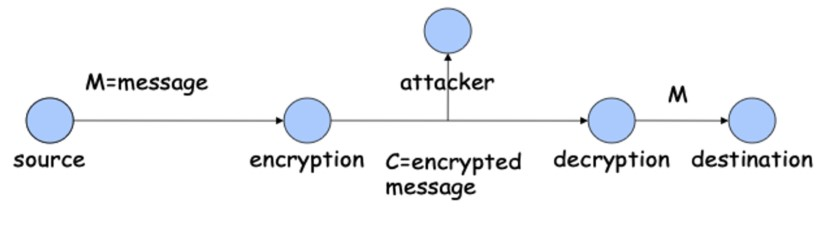
\includegraphics[scale = 1.2]{img/cl1.jpg}
        \label{cl1}
        \caption{First encryption strategy}
    \end{figure}

    An example of this type of encryption is provided by the \textit{Enigma machine}, adopted by the German militaries during World War II;

    \item The \textbf{encryption algorithm is known}, even by the attacker, but Alice and Bob share some information that is not accessible by the attacker (i.e. it travels trough a secure channel), the \textbf{encryption key}.

    \begin{figure}[h!]
        \centering
        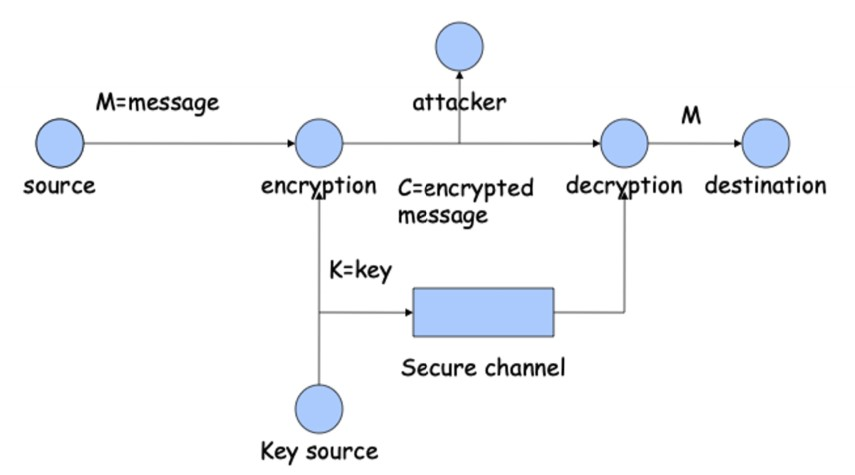
\includegraphics[scale = 1.2]{img/cl2.jpg}
        \label{cl2}
        \caption{Second encryption strategy}
    \end{figure}

    As we can see, in this case both the \textbf{encryption} and the \textbf{decryption} involve the \textbf{secret key} adopted from the source and the destination, and it is usually better than the first strategy, since:

    \begin{itemize}
        \item It is \textbf{simpler} to \textbf{distribute} only one \textbf{key}, rather than an entire encryption algorithm;
        \item If there is an attack, it is \textbf{easier} to \textbf{change key} instead of a whole algorithm.
    \end{itemize}

    For these reasons, this \textbf{second strategy} is \textbf{preferred}.
\end{enumerate}

In general, a \textbf{cryptosystem} (or a \textbf{cipher}) can be defined as a quintuple $(P,C,K,E,D)$, where:

\begin{itemize}
    \item $P$ is the set of \textbf{plaintexts}, i.e. the set of messages we want to share;
    \item $C$ is the set of \textbf{ciphertexts}, i.e. the result of the encryption applied to the plaintexts;
    \item $K$ is the set of \textbf{keys};
    \item $E: k \times P \xrightarrow{} C$ is the \textbf{encryption function}, which takes as input a key and a plaintext, and produces in output an cyphertext;
    \item $D: k \times C \xrightarrow{} P$ is the \textbf{decryption function}, which takes as input a key and a ciphertext, and produces in output a plaintext. Notice that in this case, the input $C$ of the decryption function represents the output of the encryption function.
\end{itemize}

If we consider $x \in P$ (plaintext), $y \in C$ (ciphertext) and $k \in K$, we write $E_k(x)$ and $D_k(y)$ to denote $E(k,x)$ and $D(k,y)$, i.e. the encryption and decryption under the key $k$ of $x$ and $y$, respectively. In this sense, we require that:

\begin{enumerate}
    \item $D(E_k(x)) = x$, i.e. \textbf{decrypting a ciphertext} with the right key gives the \textbf{original plaintext};
    \item Computing $k$ or $x$ given a ciphertext $y$ (which is what the attacker sees, as shown in Picture \ref{cl2}) is \textbf{unfeasible}, meaning that it is so complex that it cannot be done in a reasonable amount of time.
\end{enumerate}

It is important to underline the fact that all the invented ciphers satisfies (1), but some of them do not satisfy (2), as we will see in the following sections.

\subsection{Monoalphabetic ciphers}
We now study some of the most important monoalphabetic ciphers, i.e. ciphers in which the \textbf{letters} of the plaintext are \textbf{mapped} to ciphertext letters based on a \textbf{single alphabetic key}.

\subsubsection{Caesar cipher}
This is probably the \textbf{simplest} and most famous cipher, due to Julius Caesar. The idea is very simple: each \textbf{letter} of a message is \textbf{substituted} with the one that is \textbf{3 positions next} in the alphabet. So, for example, ‘A’ is replaced with ‘D’ and ‘M’ with ‘P’. The substitution can be represented as follows:

\begin{figure}[h!]
        \centering
        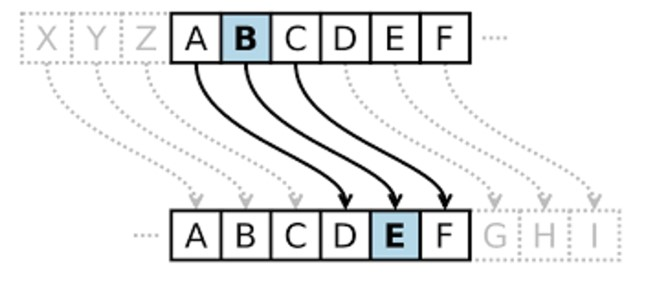
\includegraphics[scale = 1.2]{img/cl3.jpg}
        \label{cl3}
        \caption{Caesar cipher}
\end{figure}

, meaning that each letter in the top alphabet is substituted with the corresponding one in the bottom (rotated) alphabet. For example, the word HOME would be encrypted as KRPH. To \textbf{decrypt} it is enough to apply the \textbf{inverse substitution}.

\begin{figure}[h!]
        \centering
        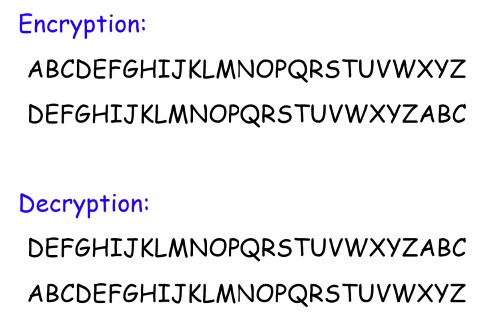
\includegraphics[scale = 1.2]{img/cl4.jpg}
        \label{cl4}
        \caption{Caesar cipher: encryption and decryption}
\end{figure}

In this case:

\begin{enumerate}
    \item The encryption is given by the substitution with the letter in 3 positions next in the alphabet;
    \item The key is 3.
\end{enumerate}

\example{We want to decrypt BHV BRX PDGH LW, and we obtain YES YOU MADE IT.}

\begin{figure}[h!]
        \centering
        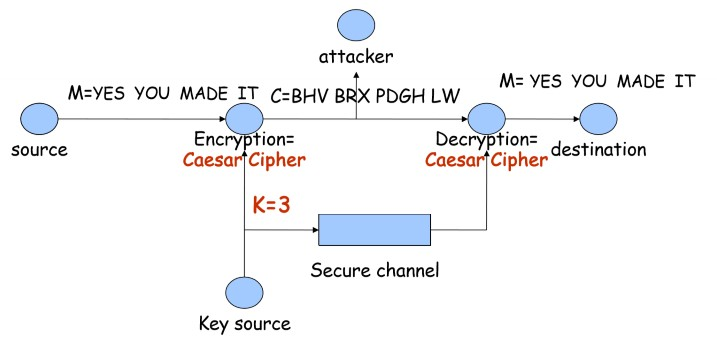
\includegraphics[scale = 1.2]{img/cl5.jpg}
        \label{cl5}
        \caption{Caesar cipher: example}
\end{figure}

Despite being extremely simple, the Ceasar cipher is clearly \textbf{insecure} for many different reasons. First of all, \textbf{once the cipher has been broken} any \textbf{previous} exchanged message is also \textbf{broken}. This is due to the fact that this cipher always works in the same way. There is a famous \textbf{principle} in cryptography, due to Auguste Kerckhoffs, that tells that a \textbf{cipher} should remain \textbf{secure} \textbf{even} if the \textbf{algorithm} becomes \textbf{public}. This is achieved by \textbf{parametrizing} ciphers on a \textbf{key}. The key can be changed and is assumed to be the only secret. This is of course fundamental if we want a cipher to scale and be used by millions of users.

Other Kerckhoffs rules (1883) are:

\begin{enumerate}
    \item The system should be, if not theoretically unbreakable, \textbf{unbreakable in practice};
    \item The \textbf{design} of a system should \textbf{not} require \textbf{secrecy}, and compromise of the system should not inconvenience the correspondents;
    \item The \textbf{key} should be \textbf{memorable} without notes and should be easily changeable;
    \item The cryptograms should be transmittable by a telegraph;
    \item The apparatus or documents should be portable and operable by a single person;
    \item The system should be easy, neither requiring knowledge of a long list of rules nor involving mental strain.
\end{enumerate}

\subsubsection{Shift ciphers}
We now consider a variant of the cipher, called \textbf{shift cipher}, which is parametrized on a key $k$, that we assume to range from 0 to 25. Intuitively, $k$ represents the number of positions in the alphabet that we \textbf{shift} each letter of (since we have 26 letters, we can perform 26 shifts, including the shift of 0 positions). Notice that in this case:

$$
P = C = K = \mathbb{Z}_{26}
$$

, i.e. the plaintexts, the ciphertexts and the keys are the set of integers from 0 to 25. Moreover:

\begin{itemize}
    \item $E_k(x) = (x+k) \mod 26$;
    \item $D_k(y) = (y-k) \mod 26$, where $y = E_k(x)$;
\end{itemize}

Notice that \textbf{Caesar cipher} represents a \textbf{subcase} of \textbf{shift cipher} when $k = 3$.

For example $k$ = 10 gives the following substitution (notice that the bottom alphabet is now shifted to the left by 10 positions):

\begin{figure}[h!]
        \centering
        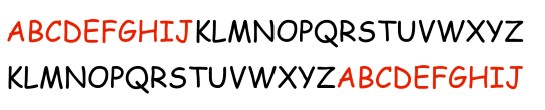
\includegraphics[scale = 1.2]{img/cl6.jpg}
        \label{cl6}
        \caption{Shift cipher: example}
\end{figure}

Does the first property hold? We have to check whether

$$
D_k(E_k(x)) = x
$$

We have that:

$$
D_k((x+k)\mod26) = [(x+k)\mod26 - k]\mod26 = x + (k-k)\mod26 = x\mod26 = x
$$

, so the \textbf{first property} holds. The previous result depends from the fact that $\mathbb{Z}_{26}$ is a group under the addition (not under multiplication). We recall that a group $<G,*>$ is a set $G$ together with a (closed) binary operation $*$ on $G$ s.t.:

\begin{itemize}
    \item The operator is associative, i.e. $(x*y)*z = x*(y*z)$;
    \item There is an element $e \in G$ s.t. $a*e = e*a = e$, the identity element;
    \item For every $a \in G$, there is an element $b \in G$ s.t. $a*b = e$, the inverse element.
\end{itemize}

Notice that $\mathbb{Z}_{26}$ is not closed under multiplication since there's no multiplicative inverse for every element in $\mathbb{Z}_{26}$.

A possible \textbf{attack} for shift cipher is the \textbf{brute force attack}, which consists in trying all the possible 26 keys (i.e. each possible shift): thus, the \textbf{second property does not hold}, since the cipher is \textbf{not secure} if the algorithm becomes public.

\subsubsection{Substitution cipher}
A possible method for overcoming the previous limitation is to consider a \textbf{generic permutation of the alphabet}, so consider a $k$ as a random permutation. Formally, 

$$
P = C = \mathbb{Z}_{26}
$$

and $k = \{\rho|\rho \text{ is a permutation of 0,..,25}\}$. Moreover:

\begin{itemize}
    \item $E_k(x) = \rho(x)$;
    \item $D_k(y) = \rho^{-1}(y)$.
\end{itemize}

An example is provided in Picture \ref{cl7}.

\begin{figure}[h!]
        \centering
        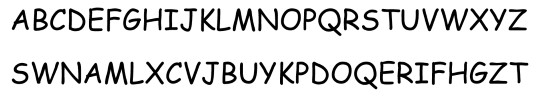
\includegraphics[scale = 1.2]{img/cl7.jpg}
        \label{cl7}
        \caption{Substitution cipher: example}
\end{figure}

Let's see if this cipher satisfy the properties:

\begin{enumerate}
    \item $D_k(E_k(x)) = x$. We have that

    $$
    D_k(\rho(x)) = \rho^{-1}(\rho(x)) = x
    $$
    , so the \textbf{first property is satisfied};
    \item Computing $k$ or $x$ given a ciphertext $y$ is unfeasible. Is the brute force technique still possible in this case? Well, we have 26! possible keys (all the possible permutations of 26 elements), which is approximately $4 * 10^{26} > 2^{88}$, which would be \textbf{unfeasible} even with powerful parallel computers.
\end{enumerate}

However, this cipher is characterized by an important \textbf{limit}, which is of being a \textbf{monoalphabetic cipher}, meaning that it \textbf{maps} a \textbf{letter} \textbf{always} to the very \textbf{same letter}. This preserves the \textbf{statistics} of the plaintext and makes it possible to \textbf{reconstruct the key} by observing the statistics in the ciphertext. For example, vowels e,a,o,i will be easy to identify as they are much more frequent than the other letters.

In this sense, if the attacker knows the used \textbf{cipher} (e.g. monoalphabetic substitution cipher) and the \textbf{language} of the plaintext (e.g. Italian), even without knowing the plaintext and the key he could be able to decrypt the plaintext, by exploiting the statistics of the language of the plaintext. For example, if he knows that the letter S appears 0 times, while letter C appears 15 times, then he can infere that letter C is a transformation of letter A, since it appears a lot of times. For each language we can build a chart of the most frequent letters/bigrams/trigrams, as showed in Picture \ref{cl8_9}.

\begin{figure}[h!]
        \centering
        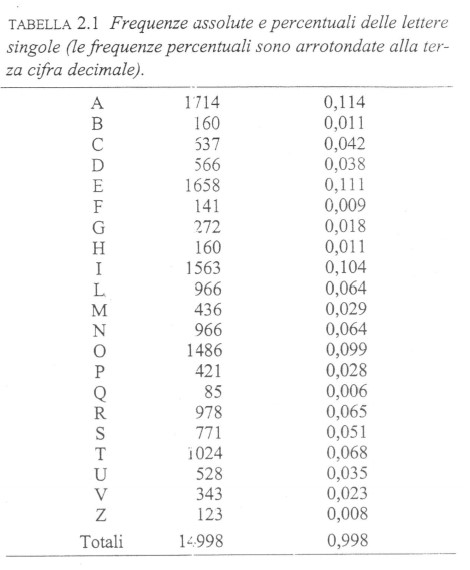
\includegraphics[scale = 1.2]{img/cl8.jpg}
        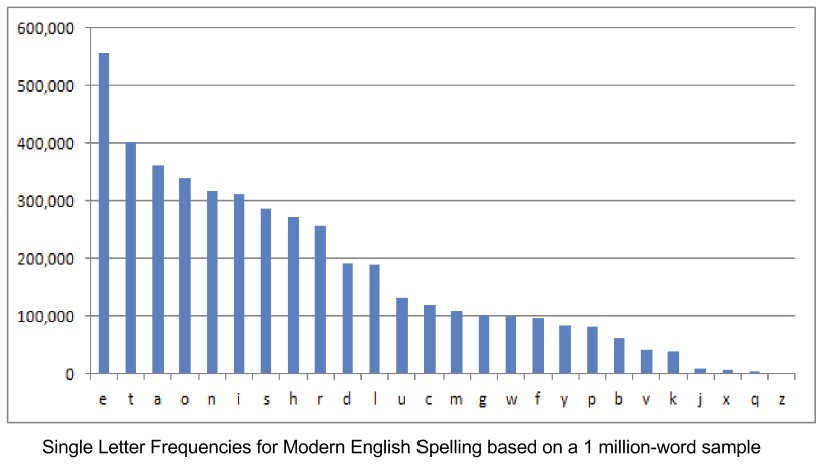
\includegraphics[scale = 1.2]{img/cl9.jpg}
        \label{cl8_9}
        \caption{Language statistics}
\end{figure}

Other deductions can be made from the fact that, for example, in Italian the frequency of letter I and L increases at the beginning of the sentences, while the one of A,E,I,O,U at the end of the words etc.. 

In this sense, a possible approach for decrypting a monoalphabetic substitution cipher could be the following:

\begin{enumerate}
    \item We \textbf{order} the letters of the ciphertext into decreasing frequencies;
    \item We \textbf{substitute} with letters in decreasing order as in the corresponding tables (depending on the language), by eventually exchanging letters with similar frequencies and by also exploiting digraphs and trigraphs frequently used,
\end{enumerate}

\subsection{Polyalphabetic ciphers}
We have seen that \textbf{monoalphabetic} ciphers are prone to \textbf{statistical attacks}, since they preserve the statistical structure of the plaintext. To overcome this issue, it is important that the same plain symbol is not always mapped to the same encrypted symbol. When this happens the cipher is called \textbf{polyalphabetic}.

\subsubsection{Vigenére cipher}
This simple polyalphabetic cipher works on \textbf{“blocks”} of $m$ letters with a key of length $m$. For example, if we consider the text "THISISAVERYSECRETMESSAEG" and the key "FLUTE", the plaintext is splitted into blocks of length 5, and the key FLUTE is repeated as necessary and used to encrypt each block, as showed in Picture \ref{poly1}.

\begin{figure}[h!]
        \centering
        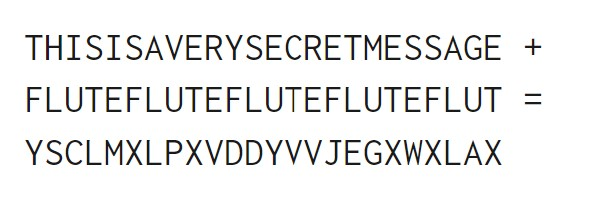
\includegraphics[scale = 1.2]{img/poly1.jpg}
        \label{poly1}
        \caption{Vigenére cipher: example}
\end{figure}

Formally, $P = C = K = \mathbb{Z}_{26}^m$, where $\mathbb{Z}_{26}^m$ is $\mathbb{Z}_{26}\times\mathbb{Z}_{26}\times\ldots\times\mathbb{Z}_{26}$, $m$ times. Encryption and decryption are defined as follows:

\begin{itemize}
    \item $E_{k1, .., km}(x_1, .., x_m) = (x_1 + k_1, .., x_m + k_m)\mod26$;
    \item $D_{k1, .., km}(y_1, .., y_m) = (y_1 - k_1, .., y_m - k_m)\mod26$
\end{itemize}

In the example above, $k_1 = \text{F}$, $k_2 = \text{L}$ etc..

The first \textbf{strength} of this cipher is that since the \textbf{number of possible keys} is $26^m$ (i.e. the number of possible keys is given by the total number of possible sequences of $m$ letters), for $m$ big enough this \textbf{prevents} \textbf{brute force attacks}. Another strength is given by the fact that \textbf{one letter} is \textbf{not always mapped} to the \textbf{same one} (unless the are at a distance that is multiple of $m$). For example the fist two letters “I” are encrypted as “C” and “M”, respectively. While the “S” in position 6 and the last one are both encrypted as “X” using the “F” of “FLUTE”. They are, in fact, at distance 15 which is a multiple of 5. Thus, the \textbf{histogram} of the \textbf{frequencies} is \textbf{flat}, and the flatness increases with the increase of the key length. 

\paragraph{Breaking Vigenére cipher: the Friedman method} Even if Vigenére cipher hides the statistic structure of the plaintext better than monoalphabetic ciphers, it still preserve most of it. There are two famous methods to break this cipher. The first is due to Friedrick Kasiski (1863) and the second to Wolfe Friedman (1920). We illustrate the latter since it is more suitable to be mechanized. Both are based on the following steps:

\begin{enumerate}
    \item Recover the \textbf{length} $m$ of the \textbf{key}. The intuition is that once we know $m$, we know that at distance $m$ we'll find the same letter of the key, thus the letters at distance $m$ form a monoalphabetic cipher;
    \item Recover the \textbf{key}.
\end{enumerate}

\textbf{STEP 1: recover \textit{m}}

The Friedman method uses statistical measures to recover the length $m$ of the key. In particular, we consider the \textbf{index of coincidence}, which is defined as:

$$
I_c(x) = \frac{\sum_{i = 1}^{26} f_i (f_i - 1)}{n (n-1)} \approx \sum_{i = 1}^{26} p_i^2
$$
, where:

\begin{itemize}
    \item $x$ represents the text for which the index of coincidence is computed;
    \item $f_i$ represents the frequency of the $i$-th letter in the text;
    \item $n$ is the length of the text;
    \item $p_i$ represents the probability of the $i$-th letter, and it is computed as $p_i = \frac{f_i}{n}$.
\end{itemize}

Intuitively, the index of coincidence measures the \textbf{probability} that \textbf{two letters}, chosen at \textbf{random} from the text $x$, are the \textbf{same}. Indeed, the index is computed by multiplying the probability that the first letter is the $i$-th ($\frac{f_i}{n}$) and the probability that the second letter is the $i$-th ($\frac{f_i - 1}{n-1}$): in this case we subtract 1 since the first letter has been already fixed).

\example{We compute the index of coincidence of the text "the index of coincidence". We have that:$$\frac{\text{c}(3 * 2) + \text{d}(2 * 1) + \text{e}(4 * 3) + \text{f}(1 * 0) + \text{h}(1 * 1) + ...}{21 * 20} = 0.0809$$}

If we consider the random text "bmqvszfpjtcsswgwvjlio", the index has value $0.0286$: as we can see, the index of coincidence of a random sentence is smaller that the one of a normal sentence. 

More specifically, notice that the \textbf{value} of the index is \textbf{minimum}, with value $1/26 \approx 0.038$, for texts composed of \textbf{letters} chosen with \textbf{uniform probability} $1/26$ while it is \textbf{maximum}, with value $1$, for texts composed of just a \textbf{single letter} repeated $n$ times. It is, in fact, a \textbf{measure} of how \textbf{non-uniformely letters} are \textbf{distributed} in a \textbf{text}. For this reason, each \textbf{natural language} has a characteristic \textbf{index of coincidence}: for English the value is approximately $0.065$. 

In general, using frequencies analysis, we saw that if \textbf{frequencies} are \textbf{flat} we have a \textbf{polyalphabetic cipher}, if we have \textbf{peaks} and valleys of frequencies we have a \textbf{monoalphabetic cipher}. If the \textbf{value} of the \textbf{index of coincidence} is \textbf{minimum} ($\approx 0.038$) we have a \textbf{polyalphabetic cipher}, if it is $\approx 0.065$ we have a \textbf{monoalphabetic cipher} (same as English, just a permutation of letters).

Now the question is: how do we recover the length $m$ of the key using the Friedman method, and in particular the concept of index of coincidence? Well, the idea is to find the length by brute-forcing, following this algorithm:

\begin{figure}[h!]
        \centering
        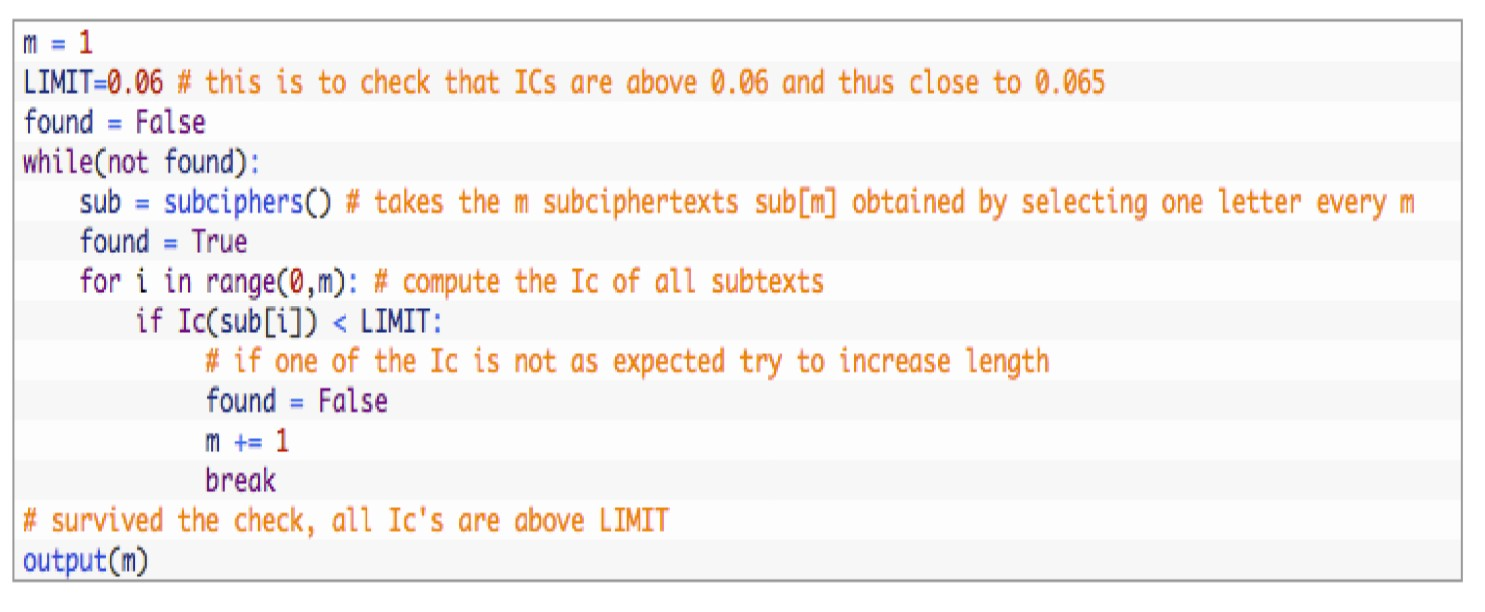
\includegraphics[scale = 0.9]{img/poly2.jpg}
        \label{poly2}
        \caption{Friedman method: estimating $m$}
\end{figure}

As we can see, the idea of the algorithm is the following:

\begin{enumerate}
    \item We \textbf{initialize} the value of $m$ to 1 (a value $m = 0$ does not make sense);
    \item We consider the $m$ \textbf{sub-ciphertexts} obtained by selecting one letter every $m$ (e.g. for $m = 2$ we get the two sub-ciphertexts composed of only the letters in odd positions and even positions, respectively);
    \item Then, we compute the \textbf{index of coincidence} of all the sub-ciphertexts, increasing the value of $m$ if the current index has a value smaller than $0.065$ (the IC of the English language). We require that the index of coincidence of all the subtexts is close to the characteristic index of the plaintext language. Typically, the bigger is the index the higher is the probability that the frequencies of the letters are close to the one of the plaintext language. It is thus enough to choose a lower bound such as 0.06 and check that the ICs are above that;
    \item The loops stops when $IC(\text{sub-ciphertext}) \geq 0.065$.
\end{enumerate}

\textbf{STEP 2: recover the key}
Once we have found the length $m$ of the key, we need to \textbf{find the key}. We consider a \textbf{text} composed of \textbf{letters} at \textbf{distance} $m$ from the first one, and the ones at distance $m$ from the second one. They have different shifts, how can we find the \textbf{relative right shift}? An example is provided in Picture \ref{poly3}.

\begin{figure}[h!]
        \centering
        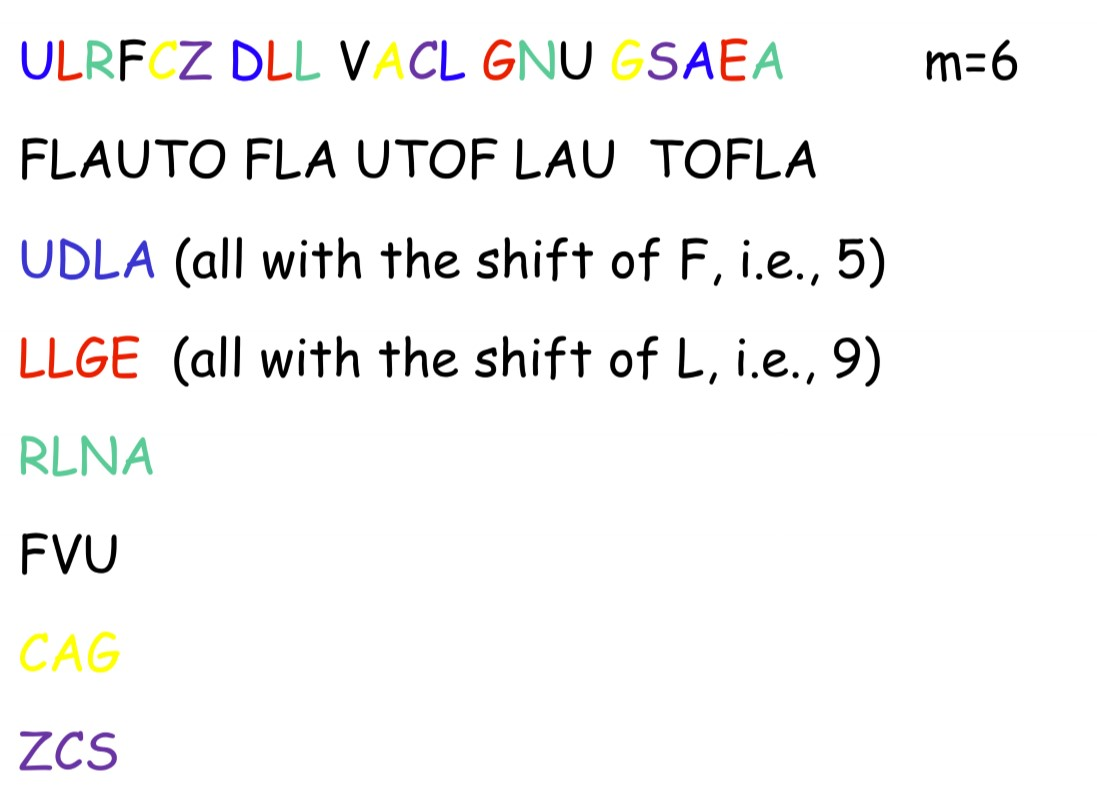
\includegraphics[scale = 0.75]{img/poly3.jpg}
        \label{poly3}
        \caption{Examples of shifts}
\end{figure}

Our goals now are:

\begin{enumerate}
    \item Determine the \textbf{shift} between the first letter of the key and the other $m-1$ letters;
    \item Determine the \textbf{first letter} (brute force on 26 possible letters) and, by exploiting the shifts we've just computed, determine the remaining letters of the key.
\end{enumerate}

We find the \textbf{relative shift} between two sub-ciphers by using the \textbf{mutual index of coincidence}, which is defined as:

$$
MI_c (x,x') = \frac{\sum_{i = 1}^{26} f_i f_i'}{n n'} = \sum_{i = 1}^{26} p_i p_i'
$$
, where:

\begin{itemize}
    \item $x$ represents the first text for which the mutual index of coincidence is computed;
    \item $x'$ represents the second text for which the mutual index of coincidence is computed;
    \item $f_i$ represents the frequency of the $i$-th letter in the text $x$;
    \item $f_i'$ represents the frequency of the $i$-th letter in the text $x'$;
    \item $n$ is the length of the text $x$;
    \item $n'$ is the length of the text $x'$;
    \item $p_i$ represents the probability of the $i$-th letter in text $x$, and it is computed as $p_i = \frac{f_i}{n}$;
    \item $p_i'$ represents the probability of the $i$-th letter in text $x'$, and it is computed as $p_i' = \frac{f_i'}{n'}$.
\end{itemize}

Intuitively, the mutual index of coincidence represents the \textbf{probability} that \textbf{two letters} taken from two texts $x$ and $x'$ are the \textbf{same}. 

The idea is to \textbf{shift one sub-cipher} until the \textbf{mutual index} of coincidence with the first sub-cipher becomes \textbf{close} to the one of the plaintext language. When this happens, we know that the applied shift is the relative shift between the two sub-ciphers and, consequently, between the corresponding letters of the key. This is encoded in the following algorithm. In fact, what we do, is to select the relative shift that maximizes the mutual index of coincidence.

\begin{figure}[h!]
        \centering
        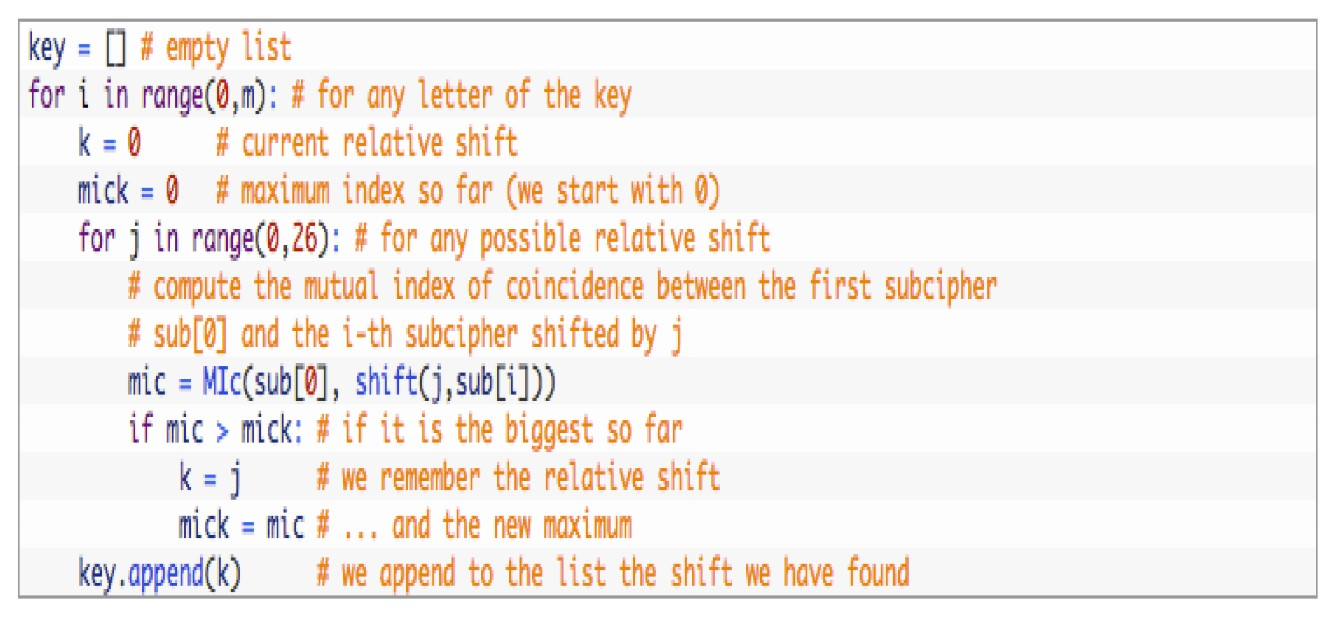
\includegraphics[scale = 0.9]{img/poly4.jpg}
        \label{poly4}
        \caption{Friedman method: finding the key}
\end{figure}

We \textbf{repeat} this \textbf{for each letter of the key}, and we obtain the \textbf{list of relative shifts}. For example key = [0,4,6,3,9] means that the second letter of the key is equal to the first plus 4 while the third is the first plus 6 and so on. The final step is to try all the possible 26 first letter of the key, giving 26 possible keys (this step could be avoided computing the MIc with a reference text written in the plaintext language).

\subsubsection{Properties}
In general, polyalphabetic ciphers are more \textbf{difficult} to be \textbf{decrypted}, but still are \textbf{not strong enough} (we presented a method for attacking Vigenére cipher).

\subsection{Known-plaintext attacks}
So far, we have considered \textbf{attackers} that \textbf{only know the ciphertext} $y$ and try to \textbf{find} either the \textbf{plaintext} $x$ or the \textbf{key} $k$. In practice, it is often the case that an \textbf{attacker} can \textbf{guess part of the plaintext}. Think of encrypted messages: a message always have a standard header in a certain format and it is often easy to guess part of the information in it. Thus if a message is split into blocks which are encrypted under the same key, it is reasonable to assume that an attacker can deduce part of the plaintext. Also, if a key is reused to encrypt many plaintexts, it can occur that in the future one of the plaintext is leaked (because its security is no more relevant). This gives the attacker knowledge of a pair $(x,y)$ \textbf{plaintext, ciphertext}.

For these reasons, in cryptography we often consider so-called \textbf{known-plaintext attacks}, i.e., we assume the attacker knows some pairs $(x’,y’), (x'',y''), ..$ of plaintexts/ciphertexts. The challenge, given $y$, is to find the relative $x$ or the $k$. We illustrate this kind of attacks on a classical cipher.

In general, the possible attacks we can consider are:

\begin{itemize}
    \item \textbf{Ciphertext-only attacks}: in a ciphertext-only attack the \textbf{attacker} is \textbf{assumed} to have access only to a set of \textbf{ciphertexts} (e.g., monoalphabetic ciphers, polyalphabetic ciphers). In this case the \textbf{limit} is that it is \textbf{easy to find} the \textbf{correspondence} between \textbf{letters} in the \textbf{plaintext} and in the \textbf{ciphertext};
    \item \textbf{Known-plaintext attacks}: the attacker knows some \textbf{pairs} $(x',y'), (x'', y''), ..$ of plaintexts/ciphertexts;
    \item \textbf{Chosen-plaintext attack (CPA)}, which presumes that the attacker can ask and obtain the \textbf{ciphertexts} for \textbf{given plaintexts};
    \item \textbf{Chosen-ciphertext attack (CCA)}, where the cryptanalyst can gather information by obtaining the \textbf{decryptions} of \textbf{chosen ciphertexts}. 
\end{itemize}

\subsubsection{The Hill cipher}
This cipher is polyalphabetic and generalizes the idea of Vigenére by introducing \textbf{linear transformations} of blocks of plaintext. 

Formally, ${\cal P} = {\cal C} = \mathbb{Z}_{26}^m$, while ${\cal K} = \{ K \ | \ K  \text{ is an invertible mod 26 } m\times m \text{ matrix} \}$. Encryption and decryption are defined as follows:

\begin{itemize}
    \item $E_k (x_1, .., x_m) = (x_1, .., x_m) K \mod 26$, i.e. we multiply the message and the matrix, modulo 26;
    \item $D_k (y_1, .., y_m) = (y_1, .., y_m) K^{-1} \mod 26$, i.e. we multiply the encrypted message and the inverse of the matrix, modulo 26.
\end{itemize}

\example{Let us assume $M = \text{message } = (x_1, x_2) = (5,9)$, and $ K = \begin{bmatrix} 5 & 11 \\8 & 3  \end{bmatrix}$. \\ To \textbf{encrypt} $M$, we have to: \begin{itemize} \item Take $M = (x_1, .., x_m)$ and $K$ which is a \textbf{matrix}; \item Compute $(x_1,...,x_m) K \mod 26$. \end{itemize} Thus, $E_k (5,9) = (5,9) * \begin{bmatrix} 5 & 11 \\ 8 & 3  \end{bmatrix} \mod 26 = (25 + 72, 55 + 27) \mod 26 = (19,4)$. \\ To \textbf{decrypt} $M$, we have to: \begin{itemize} \item Compute the \textbf{inverse} of $K$, i.e., $K^{-1}$ ($K$ is invertible); \item Compute $(y_1, .., y_m) K^{-1} \mod 26$. \end{itemize} The \textbf{inverse} of $K$ is computed as: $$ K^{-1} = \text{det}^{-1}(K) \begin{bmatrix} 3 & -11 \\ -8 & 5  \end{bmatrix} \mod 26 = \text{det}^{-1} (K) \begin{bmatrix} 3 & 15 \\ 8 & 5  \end{bmatrix} \mod 26 $$ Now, $$ \text{det}(K) = (15 - 88) \mod 26 = 5 $$, and to compute $\text{det}^{-1} (K)$ (i.e. the inverse mod 26 of 5) we need to find a number in the interval [0,25] that multiplied by 5 mod 26 gives 1. In this case the number is 21 ($5 * 21 \mod 26 = 1$). Thus, $\text{det}^{-1} (K) = 21$. Notice that it is not always the case that the multiplicative inverse modulo exists. We will discuss this more in detail when introducing public key cryptography and RSA. We now have to solve: $$ K^{-1} = \text{det}^{-1} (K) \begin{bmatrix} 3 & 15 \\ 18 & 5  \end{bmatrix} \mod 26 = 21 \begin{bmatrix} 3 & 15 \\ 18 & 5  \end{bmatrix} \mod 26 = \begin{bmatrix} 63 & 315 \\ 378 & 105  \end{bmatrix} \mod 26 = \begin{bmatrix} 11 & 3 \\ 14 & 1  \end{bmatrix} $$ Thus, $$ D_k(19,4) = (19,4) * \begin{bmatrix} 11 & 3 \\ 14 & 1 \end{bmatrix} \mod 26 = (265, 62) \mod 26 = (5,9)$$}

Assume, now, that the \textbf{attacker} knows (at least) $m$ \textbf{pairs} of plaintexts/ciphertexts, where $m$ is the block length, and his goal is to \textbf{find} the relative $x$ or $k$ given $y$. We know that:

\begin{align*}
    (y_1^1, .., y_m^1) = (x_1^1, .., x_m^1) K \mod 26 \\ 
    \hdot \\
(y_1^m, .., y_m^m) = (x_1^m, .., x_m^m) K \mod 26
\end{align*}

, where each $x^i$ represents a plaintext, and each $y^i$ represents a ciphertext. Moreover, the previous system of equations can be written as:

$$
Y = XK \mod 26
$$

, where $X = \begin{bmatrix}
x_1^1 & \hdots & x_m^1 \\
\hdots & \ddots & \hdots \\
x_1^m & \hdots & x_m^m
\end{bmatrix}$ and $Y = \begin{bmatrix}
y_1^1 & \hdots & y_m^1 \\
\hdots & \ddots & \hdots \\
y_1^m & \hdots & y_m^m
\end{bmatrix}$. 

It is now clear that if $X^{-1}$ exists, we obtain:

$$
X^{-1}Y \mod 26 = X^{-1} X K \mod 26
$$

, but $X^{-1}X = 1$, so $K = X^{-1}Y \mod26$.

The \textbf{Hill cipher} is a \textbf{linear transformation of a plaintext block} into a \textbf{cipher block}. The above attack shows that this kind of \textbf{transformation} is \textbf{easy to break} if enough \textbf{pairs} of \textbf{plaintexts} and \textbf{ciphertexts} are \textbf{known}. \textbf{Modern ciphers}, in fact, always contain a \textbf{non-linear component} to prevent this kind of attacks.

\example{Assume that the attacker has the pairs $(5,9) \xrightarrow{} (19,4)$ and $(2,5) \xrightarrow{}(24,11)$, and $m = 2$. How can we find $K$? Firstly, we need to compute $X^{-1}$: if this matrix exists, we can derive $K$ from the formula above. \begin{equation*} \begin{align*} X^{-1} &= \text{det}(X)^{-1} \begin{bmatrix} 5 & -9 \\ -2 & 5  \end{bmatrix} \mod 26 \\ &= \text{det}(X)^{-1} \begin{bmatrix} 5 & 17 \\ 24 & 5  \end{bmatrix} \mod 26 \\ &= 15  \begin{bmatrix} 5 & 17 \\ 24 & 5  \end{bmatrix} \mod 26 \\ &= \begin{bmatrix} 23 & 21 \\ 22 & 23  \end{bmatrix}     \end{align*} \end{equation*} Then, $K = X^{-1}Y \mod 26 = \begin{bmatrix} 23 & 21 \\ 22 & 23  \end{bmatrix} \begin{bmatrix} 19 & 4 \\ 24 & 11 \end{bmatrix} \mod 26 = \begin{bmatrix} 5 & 11 \\ 8 & 3 \end{bmatrix}$}

\subsection{Euclidean algorithm}
We now consider an \textbf{algorithm} for computing in an \textbf{efficient} way the operation of \textit{inverse modulo $n$}. We begin by introducing the \textbf{Euclidean algorithm}, which is used to computed $\text{gcd}(c,d)$ represented in Picture \ref{eu1}.

\begin{figure}[h!]
        \centering
        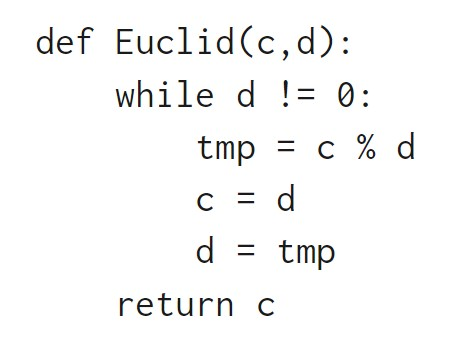
\includegraphics[scale = 0.9]{img/eu1.jpg}
        \label{eu1}
        \caption{Euclidean algorithm}
\end{figure}

In this case, the idea is that, to compute $\text{gcd}(c,d)$, when $d \neq 0$, we can compute $\text{gcd}(d,c \mod d)$, since it can be easy seen that they're the same.

\example{$\text{gcd}(5,15) = 5$}.

This algorithm terminates in $O(k^3)$, given that the \textbf{number of iterations} is $O(k)$. This latter fact can be proved by observing that every 2 steps we at least halve the value $d$. Assume by contradiction that after one step this is not true, i.e., $c \mod d > \frac{d}{2}$. Next step will compute $d \mod (c \mod d) = d - (c \mod d) < \frac{d}{2}$ giving the thesis. We know that halving leads to a logarithmic complexity, i.e., linear with respect to the number of bits $k$.

We now \textbf{extend} the \textbf{algorithm} so to compute the \textbf{inverse modulo} $d$ whenever $gcd(c,d)=1$. We substitute the computation of $c\mod d$ with:

$$
q = c/d
$$

, i.e. an integer division, and

$$
\text{tmp} = c - qd
$$

, which represents the operation $c \mod d$.

\example{$12 \mod 5 = 2$, $q = \frac{12}{5}$ and $\text{tmp} = 12 - 2*5 = 2$.}

We add two extra variables $e$ and $f$ and we save the initial value of $d$ in $d_0$, as follows:

\begin{figure}[h!]
        \centering
        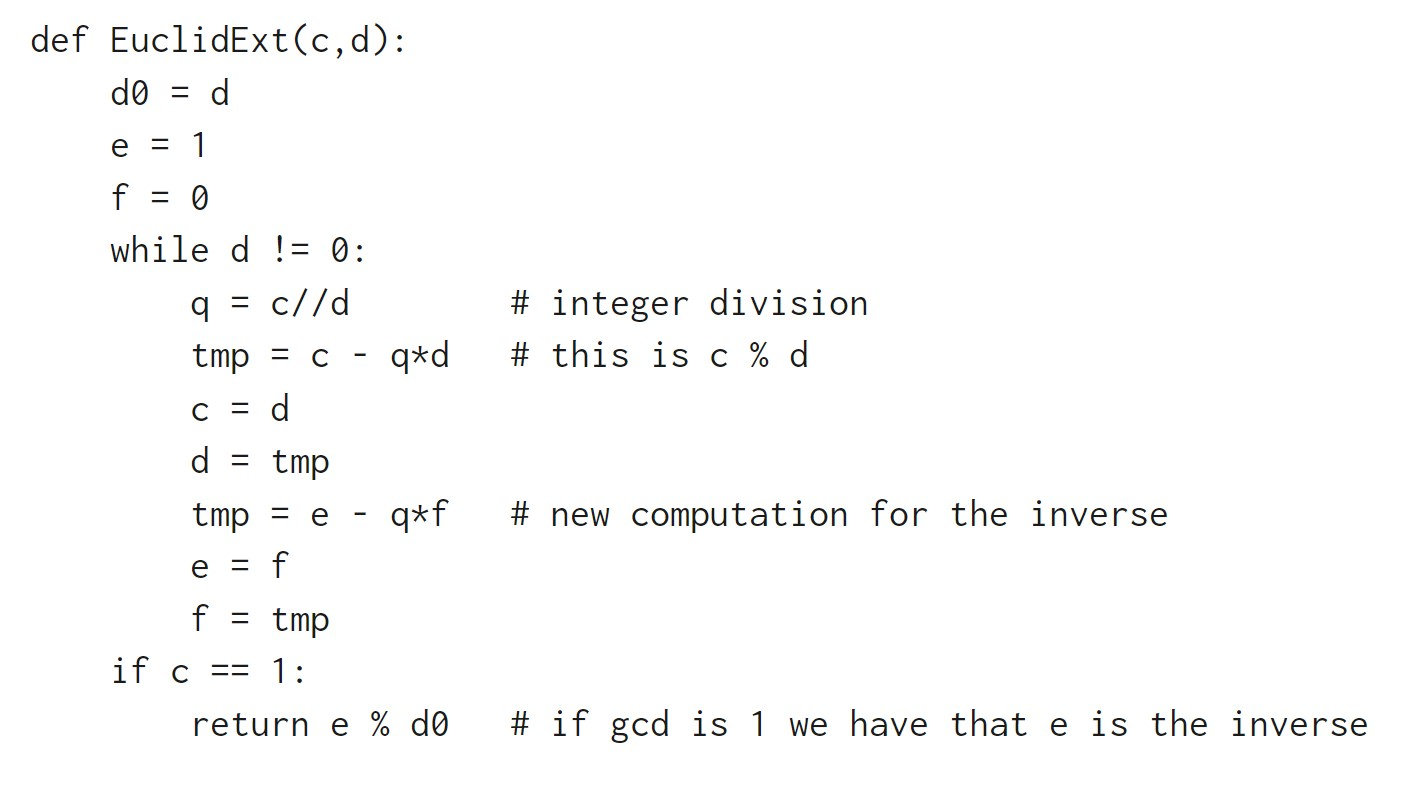
\includegraphics[scale = 0.9]{img/eu2.jpg}
        \label{eu2}
        \caption{Extended euclidean algorithm}
\end{figure}

\example{The inverse between 5 and 17 can be computed using $\text{EuclidExt}(5,17) = 7$.}

\subsection{Stream ciphers}
So far, we have illustrated cryptosystems that “reuse” the same key to encrypt letters or blocks of the plaintext. This is usually referred to as \textbf{block ciphers}.

\begin{figure}[h!]
        \centering
        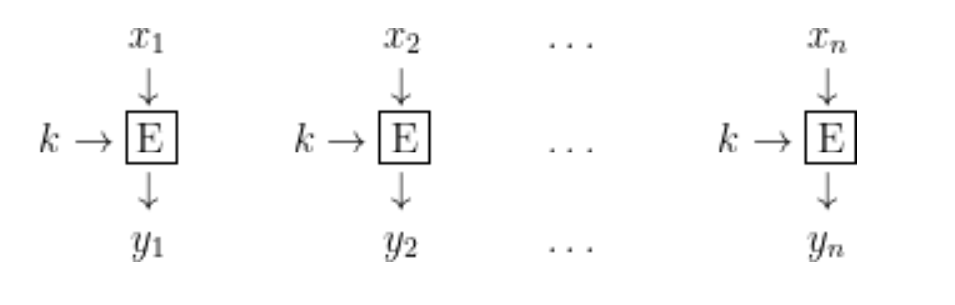
\includegraphics[scale = 1.0]{img/stream1.png}
        \label{stream1}
        \caption{Block cipher}
\end{figure}

This scheme can be \textbf{generalized} by considering a \textbf{stream of keys} instead of a fixed one. Let $z_1, z_2, \ldots, z_n$ be such a stream. The idea is to \textbf{encrypt} the \textbf{first letter} of the plaintext with $z_1$, the \textbf{second} with $z_2$ and so on. It does not matter much if we encrypt a letter or a block, the important difference is that the used key is always different.

\begin{figure}[h!]
        \centering
        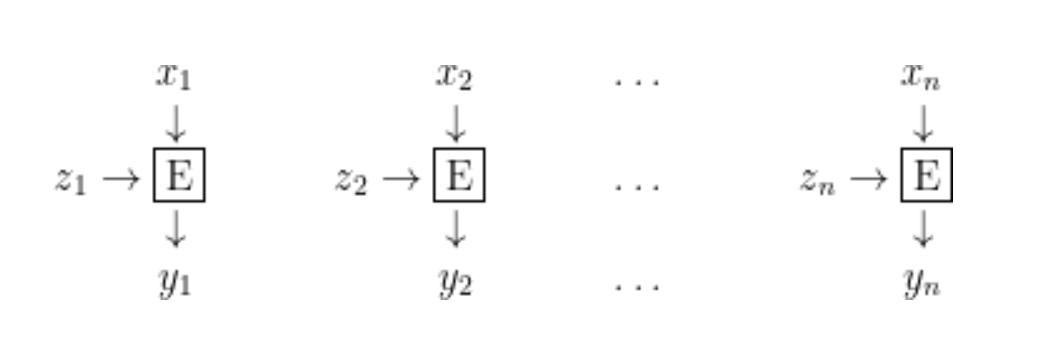
\includegraphics[scale = 1.0]{img/stream2.png}
        \label{stream2}
        \caption{Cipher using different keys}
\end{figure}

Having a \textbf{different key} for \textbf{each letter} or block of the plaintext is of course \textbf{appealing} but \textbf{not} much \textbf{practical}. The stream of key is thus usually derived starting from an initial key $k$. To make the \textbf{stream more complex} it can also \textbf{depend} on \textbf{previous part of the plaintext}. In general we say that 

$$z_i = f_i(k,x_1,\ldots,x_{i-1})$$

, i.e. the $i$-th key depends on $k$ and on the previous $i-1$ letters (or blocks).

To understand why a key $z_i$ cannot depend on plaintexts with indexes greater than or equal to $i$, it is useful to reason on the decryption scheme:

\begin{figure}[h!]
        \centering
        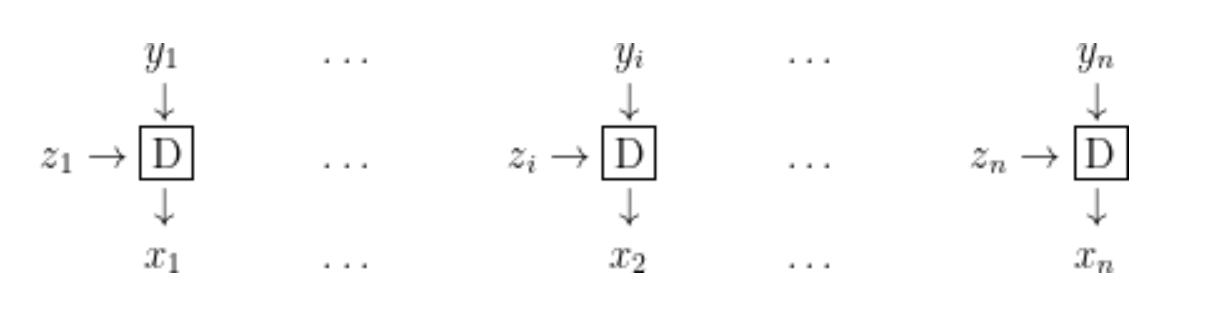
\includegraphics[scale = 1.0]{img/stream3.png}
        \label{stream3}
        \caption{Decryption of a cipher using different keys}
\end{figure}

Now, $z_1 = f_1(k)$ meaning that we can compute it with not knowledge of the plaintext. To compute $z_2 = f_2(k,x_1)$, instead, we need to know $x_1$. As a consequence, we have to decrypt $y_1$ with $z_1$ before computing $z_2$. Once we have this key we can decrypt $x_3$ and compute $z_3$, and so on. The values are thus computed in the following sequence: $z_1,x_1,z_2,x_2, \ldots, z_n,x_n$. It should be evident, now, that we cannot let $z_i$ depend, e.g., on $x_i$ as we would need that plaintext to compute the key.

Notice that \textbf{block ciphers} are, clearly, a \textbf{simple instance} of \textbf{stream ciphers} where $z_i = k$ for all $i$. It is also useful to classify these ciphers depending on certain properties of the key stream:

\begin{itemize}
    \item \textbf{Periodic} stream ciphers;
    \item \textbf{Synchronous} stream ciphers;
    \item \textbf{Asynchronous} stream ciphers;
\end{itemize}

\subsubsection{Periodic stream ciphers}
A stream cipher is \textbf{periodic} if its key stream has the following form $z_1,z_2,\ldots,z_d,z_{1},z_2,\ldots,z_d,z_1\ldots$, i.e., if it \textbf{repeats} after $d$ steps.

Note that \textbf{Vigenére ciphers} can be seen as a \textbf{stream cipher} acting on \textbf{single letters} and with a \textbf{periodic key stream}. For example, if we want to formalize the cipher giving $({\cal P},{\cal C},{\cal K},E,D)$  and defining the key stream $z_i$, we have that:

\begin{itemize}
    \item $E_{z_i}(x_i)=(x_i+z_i) \mod 26$;
    \item $D_{z_i}(y_i)=(y_i-z_i) \mod 26$;
    \item $z_i = k_{i \mod m}$.
\end{itemize}

\subsubsection{Synchronous stream ciphers}
A stream cipher is \textbf{synchronous} if its \textbf{key stream does not depend on plaintexts}, i.e., $z_i = f_i(k)$ for all $i$. When this happens, we have that the key stream can be generated starting from $k$ and independently on the plaintext. This is particularly useful to improve efficiency: we do not need to obtain $x_{i}$ to compute $z_{i+1}$. In fact, the key stream can be generated offline, before the actual ciphertext is received.

As an example, \textbf{Vigenére ciphers} can be seen as a \textbf{synchronous stream cipher}.

\subsubsection{Asynchronous stream ciphers}
This is the general case where $z_i = f_i(k,x_1,\ldots,x_{i-1})$. As mentioned above, we need to decrypt and compute the keys stream at the same time, as a key can depend on previous plaintexts. 

We give a simple example of a cipher of this class, called \textbf{Autokey}. We let ${\cal P}={\cal C}={\cal K}=\mathbb{Z}_{26}$. $E_z(x) = x+z \mod 26$ and $D_z(y) = y-z \mod 26$, i.e., \textbf{encryption} and \textbf{decryption} are exactly as in a \textbf{shift cipher}. The key stream is defined as $z_1 = k$ and $z_i = x_{i-1}$ for $i\geq 2$, meaning that the first key in the stream is the initial key k while the next keys are the same as the previous plaintext.

\begin{figure}[h!]
        \centering
        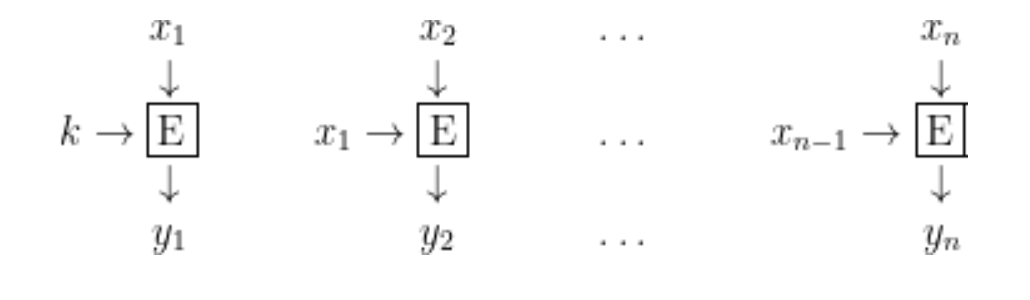
\includegraphics[scale = 1.0]{img/stream4.png}
        \label{stream4}
        \caption{Autokey cipher}
\end{figure}

\example{Consider the autokey cipher, and assume that the plaintext is the word "networksecurity", what is the encryption using $k = 5$ (recall: $E_z(x) = x+z \mod 26$)? The corresponding numbers are 13, 4, 19, 22, 14, 17, 10, 18, 4, 2, 20, 17, 8, 19, 24, so the encryption is $z_1 = 5$, $z_2 = x_1 = 13$, $z_3 = x_2 = 4$ etc.., so the result numbers are 18, 17, 23, 15, 10, 5, 1, 2, 22, 6, 22, 11, 25, 1, 17, and the corresponding ciphertext is SRXPKFBCWGWLZBR. For the encryption, we have that $D_z(y) = y-z \mod 26$, so we can use $k = 5$ to find the first letter $x_1$ of the plaintext: $x_1 = (18-5) \mod 26 = 13$. Then, we can use $x_1$ as a key to find $x_2$ : $x_2 = (17-13) \mod 26 = 4$ etc..}

Notice that the \textbf{autokey} cipher is \textbf{insecure}, since there are only 26 different keys.

\subsection{Perfect ciphers}
We now discuss a \textbf{theoretical result} on the security of cryptosystems. We ask whether \textbf{perfect ciphers} exists, i.e., ciphers that can never be broken, even with after an unlimited time (informal definition). Interestingly, we will see that these ideal ciphers \textbf{exist} and \textbf{can be implemented in practice} but they are, in fact, \textbf{unpractical}. The theory, developed by \textbf{Claude Shannon}, assumes an \textbf{only-ciphertext} model of the \textbf{attacker}, i.e., the attacker only knows the ciphertext $y$ and tries to find plaintext $x$ or key $k$.

Another informal definition of perfect cipher is the following: a cipher system is said to offer perfect secrecy if, on \textbf{seeing} the \textbf{ciphertext} the interceptor gets \textbf{no extra information} about the \textbf{plaintext} than he had before the ciphertext was observed. In a cipher system with perfect secrecy the interceptor is “forced” to guess the plaintext.

\subsubsection{Probability distribution}

We call:

\begin{itemize}
    \item $p_{\cal P}(x)$ the \textbf{probability} of a \textbf{plaintext} $x$ to occur;
    \item $p_{\cal K}(k)$ the \textbf{probability} of a certain \textbf{key} $k$ to be used as encryption key.
\end{itemize}

These two probability distributions induce a \textbf{probability distribution} on the \textbf{ciphertexts}. In fact, given a plaintext and a key there exists a unique corresponding ciphertext. We can compute such a probability distribution as follows:

$$
p_{\cal C}(y) = \displaystyle \sum_{k \in {\cal K}, \exists x . E_k(x)=y} {p_{\cal K}(k) p_{\cal P}(D_k(y))}
$$

Given a \textbf{ciphertext} $y$ we look for \textbf{all the keys} that \textbf{can give} such a \textbf{ciphertext} from some \textbf{plaintext} $x$. We then sum the probability of all such keys times the probability of the corresponding plaintext.

\example{Consider the following toy-cipher with $P = \{a,b\}$, $K = \{k_1,k_2\}$, $C = \{1,2,3\}$. The encryption is defined by the following table: \begin{table}[h!] \centering\begin{tabular}{c|c|c}$E$ & $a$ & $b$ \\\hline $k_1$ & 1 & 2 \\$k_2$ & 2 & 3\end{tabular}\caption{Caption}\label{tab:my_label}\end{table} We now let $p_p(a) = 3/4$, $p_p(b) = 1/4$, $p_k(k_1) = p_k(k_2) = 1/2$. Let us now compute $p_c(1)$: $$ p_c(y) = \sum_{k \in \mathcal{K}, \exists x . E_k (x) = y} p_{k} (k) p_p(D_k(y)) $$ Thus, $p_c(1) = p_k(k_1) p_p(D_k(1)) = 1/2 * 3/4 = 3/8$.}

\subsubsection{Conditional probability}
We can also compute the \textbf{conditional probability} of a \textbf{ciphertext} $y$ with respect to a \textbf{plaintext} $x$. This gives a measure of how likely is a certain ciphertext once we fix a plaintext.

$$p_{\cal C}(y|x) = \displaystyle \sum_{k \in {\cal K}, E_k(x)=y} {p_{\cal K}(k) }$$

It is simply the sum of the probability of all keys giving $y$ from $x$.

\example{The conditional probability of ciphertext 1 w.r.t. the two plaintexts $a$ and $b$ is: $$p_{\cal C}(1|a) = \displaystyle \sum_{k \in {\cal K}, E_k(x)=y} {p_{\cal K}(k) } = p_{\cal K}(k1) = 1/2$$ $$p_{\cal C}(1|b) = \displaystyle \sum_{k \in {\cal K}, E_k(x)=y} {p_{\cal K}(k) } =0$$ Notice, in particular, that 1 can never be obtained from $b$.}

Once we have these values, the idea is to compute the \textbf{conditional probability} of a \textbf{plaintext} with respect to a \textbf{ciphertext}. This is very related to the \textbf{security} of the cipher, since it is a measure of how likely is a plaintext once a ciphertext is observed (which is what the attacker is usually interested to know). Interestingly, this conditional probability can be computed through that \textbf{Bayes theorem}:

$$p_{\cal P}(x|y) =\displaystyle \frac{p_{\cal P}(x)p_{\cal C}(y|x)}{p_{\cal C}(y)}$$

This conditional probability is quite useful when we'll prove that a cipher is perfect if $\forall x,y$, $p_{\cal P}(x|y) = p_{\cal P}(x)$.

\example{We can now compute the probabilities of plaintexts $a$ and $b$ with respect to ciphertext 1. We obtain: $$p_{\cal P}(a|1) = \displaystyle \frac{p_{\cal P}(a)p_{\cal C}(1|a)}{p_{\cal C}(1)} = \displaystyle \frac{3/4 \times 1/2}{3/8} = 1$$ $$p_{\cal P}(b|1) = \displaystyle \frac{1/4 \times 0}{3/8} = 0$$ Thus, when observing 1 we are sure it is plaintext $a$ and that it's not plaintext $b$, meaning that this cipher is completely insecure. The same happen if we compute the probabilities of $a$ and $b$ when observing 3 (in this case we're sure that it is plaintext $b$ and not $a$, i.e. $p_{\cal P}(b|3) = 1$ and $p_{\cal P}(a|3) = 0$). For ciphertext 2 we have an interesting, less extreme, situation. We obtain, in fact, $p_{\cal P}(a|2) = 3/4$ and $p_{\cal P}(b|2) = 1/4$, thus $a$ is more likely than $b$ when 2 is observed. This might suggest that even for this ciphertext the attacker gains information (even if partial) about the plaintext. However, it is important to notice that $p_{\cal P}(a) = 3/4, p_{\cal P}(b) = 1/4$, i.e., that the probability of the two plaintexts, when 2 is observed, is exactly the one they occur in a message. In fact, observing 3 does not change anything.}

\subsubsection{Formal definition}
We now give the definition of perfect cipher:

\definition{Perfect cipher}{A cipher is \textbf{perfect} if and only if $p_{\cal P}(x|y)=p_{\cal P}(x)$ for all $x \in {\cal P}$ and $y \in {\cal C}$.}

Intuitively, a cipher is perfect if \textbf{observing} a \textbf{ciphertext} $y$ gives \textbf{no information} about any of the possible \textbf{plaintexts} $x$. 

The cipher in the example is far from being perfect, but it satisfies the above definition for ciphertext 2. Concerning ciphertext 3, we have that $p_{\cal P}(a) = 3/4 \neq p_{\cal P}(a|3) = 0$, and $p_{\cal P}(b) = 1/4 \neq p_{\cal P}(b|3) = 1$, so the property does not hold.

Another possible definition is the following: if we consider a completely \textbf{bipartite graph} composed by \textbf{plaintexts} and \textbf{ciphertexts}, as the one in Picture \ref{perfect1}, a cipher is defined as \textbf{perfect} if there is some \textbf{key} that \textbf{maps} any \textbf{message} to any \textbf{ciphertext} with \textbf{equal probability}. In this sense, the weights of the graph will all have the same weight equal to $1/n$. 

\begin{figure}[h!]
        \centering
        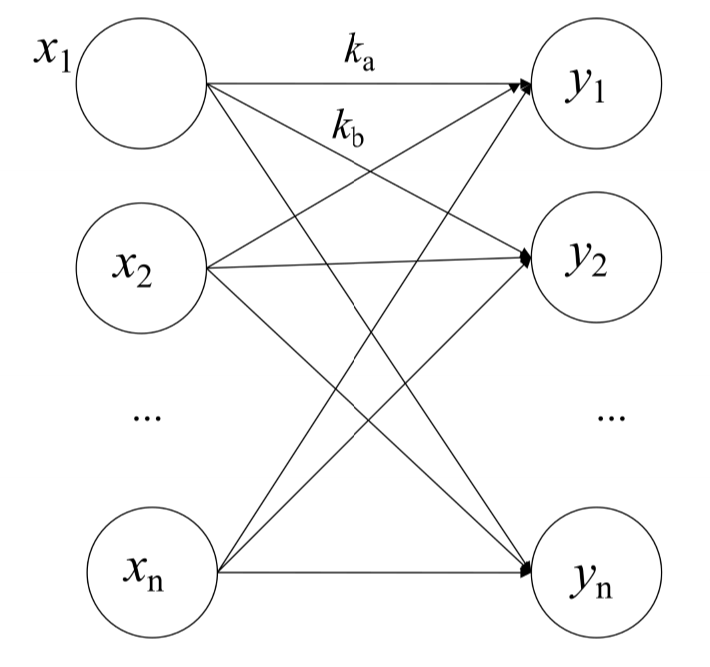
\includegraphics[scale = 0.65]{img/perfect1.png}
        \label{perfect1}
        \caption{Completely bipartite graph}
\end{figure}

\underline{Exercise}: prove that shift cipher with $p_{\cal K}(k) = \frac{1}{|{\cal K}|}=\frac{1}{26}$, i.e., with keys picked at random for each letter of the plaintext, is a perfect cipher. In other words, if we change key any time (not feasible in practice) and we encrypt a letter, then the shift cipher becomes perfect, i.e. unbreakable.

\underline{Solution}: the idea for solving this exercise is to rely on the formal definition we gave above. By using the conditional probability, if we show that $p_{\cal C}(y|x) = p_{\cal C}(y)$ for every $x$ and $y$, then $p_{\cal P}(x|y) = p_{\cal P}(x)$ for every $x$ and $y$, so the cipher is perfect. 

We recall that a shift cipher is defined as:

\begin{itemize}
    \item ${\cal P}={\cal C}={\cal K}=\mathbb{Z}_{26}$;
    \item $E_k(x) = (x+k) \mod 26$;
    \item $D_k(y) = (y-k) \mod 26$.
\end{itemize}

We compute the probability of a generic ciphertext $y$ as:

\begin{array}{rcl} p_{\cal C}(y) &=&\displaystyle \sum_{k \in {\cal K}, \exists x . E_k(x)=y} {p_{\cal K}(k) p_{\cal P}(D_k(y))}\\&=&\displaystyle \frac{1}{26}\sum_{k \in {\cal K}, \exists x . E_k(x)=y} { p_{\cal P}(D_k(y))}\\&=&\displaystyle \frac{1}{26}\sum_{k \in {\cal K}} { p_{\cal P}(y-k \mod 26)}\\&=&\displaystyle \frac{1}{26}\sum_{x \in {\cal P}} { p_{\cal P}(x)}=\frac{1}{26}\end{array}

Notice that:

\begin{itemize}
    \item The first step comes from the fact that each $p_{\cal K}(k)$ is independent of we key we choose, since it is a constant value equal to $\frac{1}{26}$;
    \item The last two steps hold since for each key $k$, we always have a plaintext that gives $y$ when encrypted under $k$. This plaintext is exactly $y-k \mod 26$. So the constraint $\exists x . E_k(x)=y$ always holds and $D_k(y) = y-k \mod 26$;
    \item Then, it is sufficient to observe that $y-k \mod 26$ for all possible keys gives exactly the set of all possible plaintexts ${\cal P}$ and the sum of all their probabilities gives 1.
\end{itemize}

We can now compute

$$p_{\cal C}(y|x) = \displaystyle \sum_{k \in {\cal K}, E_k(x)=y} {p_{\cal K}(k) } = p_{\cal K}(y-x \mod 26) = \frac{1}{26}$$

Here it is enough to observe that, given $x$ and $y$, there exists a unique key that encrypts $x$ as $y$, which is precisely $y-x\mod 26$ (derived from $y = (x+k) \mod 26$). 

Now Bayes theorem gives:

$$p_{\cal P}(x|y) =\displaystyle \frac{p_{\cal P}(x)p_{\cal C}(y|x)}{p_{\cal C}(y)}=\frac{p_{\cal P}(x)\frac{1}{26}}{\frac{1}{26}} = p_{\cal P}(x)$$

which gives the thesis.

We have seen that if we change key any time we encrypt a letter, a cipher as simple as the shift cipher becomes perfect, i.e., unbreakable. We now present two general results that, in fact, show that this strong requirement is indeed necessary and we cannot hope to develop perfect ciphers without it.

\subsubsection{Important theorems}
\theoremNum{1}{Let $p_{\cal C}(y)>0$ for all $y$. A cipher is perfect \textbf{only if} $|{\cal K}| \geq |{\cal P}|$.}

The theorem states a \textbf{necessary condition} of a cipher to be perfect: it must be that the number of keys is at least the same as the number of plaintexts. In other words:

$$
\text{perfect cipher } \xrightarrow{} |\cal K| \geq |\cal P| 
$$

and, conversely,

$$
|K| < |P| \xrightarrow{} \text{ not perfect cipher}
$$

Thus, besides the formal definition, we have a very easy way of proving that the cipher is not perfect

\textit{Proof}: we first notice that by Bayes theorem we have that a cipher is perfect if an only if $p_{\cal C}(y|x)=p_{\cal C}(y)$ for all $x \in {\cal P}$ and $y \in {\cal C}$. If we fix $x$ we obtain that for each $y$, $p_{\cal C}(y|x)=p_{\cal C}(y)>0$ meaning that there exists at least one key $k$ such that $E_k(x) = y$ (otherwise we would have $p_{\cal C}(y|x)=0$). Notice also that all such keys are different since $E_k$ is a function and we have fixed $x$. In fact, $x$ cannot be mapped to two different ciphertexts by the same key (otherwise $E_k$ would not be a function). Thus we have at least one key for each ciphertext meaning that $|{\cal K}| \geq |{\cal C}|$. Since, for any cipher, $E_k$ injects the set of plaintexts into the set of ciphertext, we also have $|{\cal C}| \geq |{\cal P}|$, which gives the thesis $|{\cal K}| \geq |{\cal P}|$.

\theoremNum{2}{Let $|{\cal P}| = |{\cal C}| = |{\cal K}|$. A cipher is perfect \textbf{if and only if}: \begin{enumerate}\item $p_{\cal K}(k) = \frac{1}{|{\cal K}|} \quad \forall k \in {\cal K}$;\item For each $x \in {\cal P}$ and $y \in {\cal C}$ there exists exactly one key $k$ such that $E_k(x)=y$.\end{enumerate}}

Intuitively, the theorem states that for a cipher to be \textbf{perfect} (under the hypothesis that the size of the set of plaintexts, ciphertexts and key is the same) \textbf{keys} should be \textbf{picked at random} for any \textbf{encryption} and each plaintext is mapped into each ciphertext through a unique key.

Conversely, in order to show that a cipher is not perfect, we need to show that either condition (1) or (2) does not hold.

\textit{Proof}: we prove that a perfect cipher implies the two above conditions. We leave the other side of the implication as an exercise. In Theorem 1 we have seen that, for perfect ciphers, if we fix $x$ we obtain that for each $y$ that $p_{\cal C}(y|x)=p_{\cal C}(y)>0$ meaning that there exists at least one key $k$ such that $E_k(x) = y$ and all of these keys are different. Thus we have $|{\cal K}| \geq |{\cal C}|$. In this theorem we have assumed $|{\cal K}| = |{\cal C}|$, meaning that all of these keys k are unique (otherwise we would have $|{\cal K}| > |{\cal C}|$). Since this holds for each $x$ and $y$ we have proved condition 2. To prove condition 1, it is enough to notice that $p_{\cal C}(y|x)=p_{\cal K}(k)$, i.e., the probability of $y$ given $x$ is equal to the probability of the unique key $k$ that encrypts $x$ into $y$. Thus, $p_{\cal K}(k) = p_{\cal C}(y|x)=p_{\cal C}(y)$ (only one key $k$ maps $x$ into $y$). If we fix $y$ and we consider all possible plaintexts $x$ we obtain all possible keys $k$ and for all of them it holds $p_{\cal K}(k) =p_{\cal C}(y)$, with $p_{\cal C}(y)$ constant. Given that the sum of the probability of all keys must be 1, we obtain $p_{\cal K}(k) = \frac{1}{|{\cal K}|}$ which proves condition 1.

\subsubsection{The one-time-pad}
We conclude giving a famous \textbf{example of a perfect cipher} that has been used in practice. This cipher has been used for the telegraph and is a binary variant of Vigenére with keys picked at random. More precisely we have ${\cal P} = {\cal C}= {\cal K} = \mathbb{Z}_2^d$ (i.e. plaintext, ciphertext and keys can be either 0 or 1, i.e. binary) with $p_{\cal K}(k) = \frac{1}{|{\cal K}|} = \frac{1}{2^d}$ for all $k \in {\cal K}$. Encryption is defined as $E_{(k_1, \ldots, k_d)}(x_1,\ldots,x_d) = (x_1 \oplus k_1, \ldots, x_d \oplus k_d)$ where $\oplus$ is the bitwise XOR operation. We recall that the XOR operation is defined as follows: 

$$
101 \text{ XOR } 011 = 110
$$

We notice that the premise of Theorem 2 holds (set sizes are the same by definition of the cipher). Also condition 1 holds, i.e., $p_{\cal K}(k) = \frac{1}{|{\cal K}|}$ by definition of the cipher. We only need to prove condition 2. Let $x \in {\cal P}$ and $y \in {\cal C}$. We have that the unique key giving $y$ from $x$ is computed as $x \oplus y$, i.e., $(x_1 \oplus y_1, \ldots, x_d \oplus y_d)$. We thus conclude that the cipher is perfect.

Despite being a perfect cipher, we notice how one-time-pad is pretty unfeasible in practice, since it needs to change the key each time.

\subsubsection{Recap}
Shannon theory on perfect ciphers shows that such ideal ciphers exist but require as many keys as the possible plaintexts, and keys need to be picked at random for each encryption. Even if this makes such ciphers unpractical, the one-time-pad has been used for real transmission. The setup consisted of two identical books with thousands of  “random” keys. Each key was used once (from which the name one-time). Once the book had been used completely, new shared books were necessary.

\newpage
\subsection{Exercises}

\begin{enumerate}
    \item Decrypt the following ciphertext using substitution cipher (the language is English):

    \begin{figure}[h!]
        \centering
        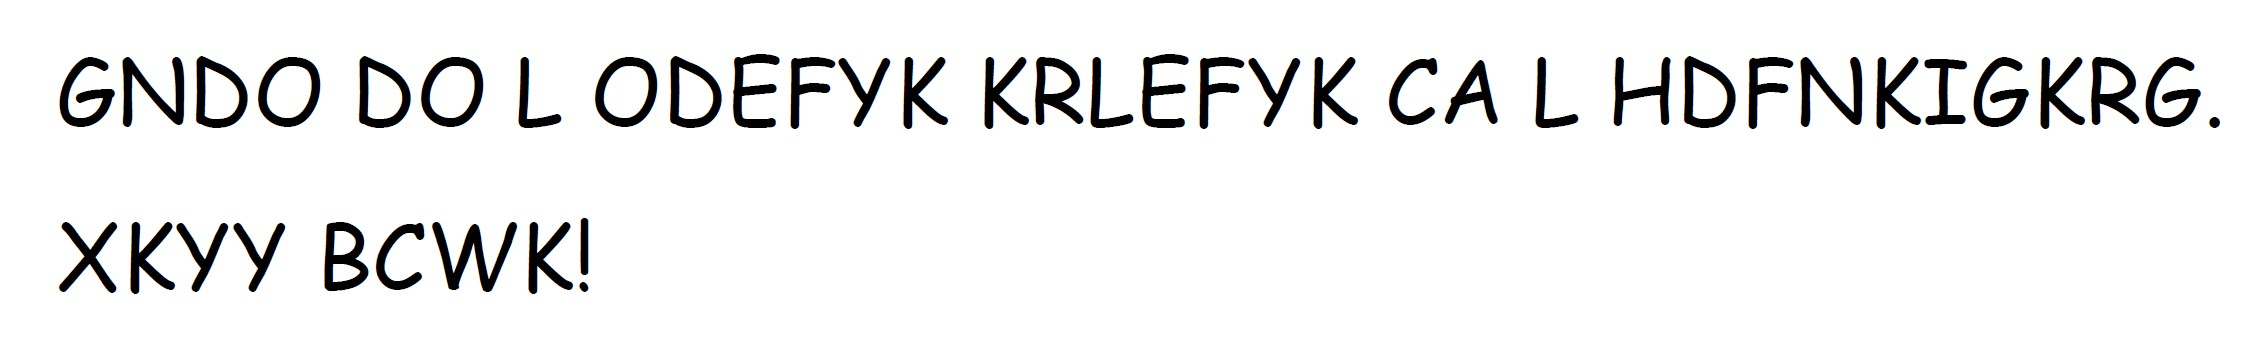
\includegraphics[scale = 0.41]{img/ex1.jpg}
        \label{ex1}
        % \caption{Friedman method: finding the key}
    \end{figure}

    \item Decrypt the following ciphertext using Vigenére cipher (the key is "FLUTE"): STWXXWJ;

    \item Write a program that decrypts the following ciphertext (Vigenére cipher):

    \begin{figure}[h!]
        \centering
        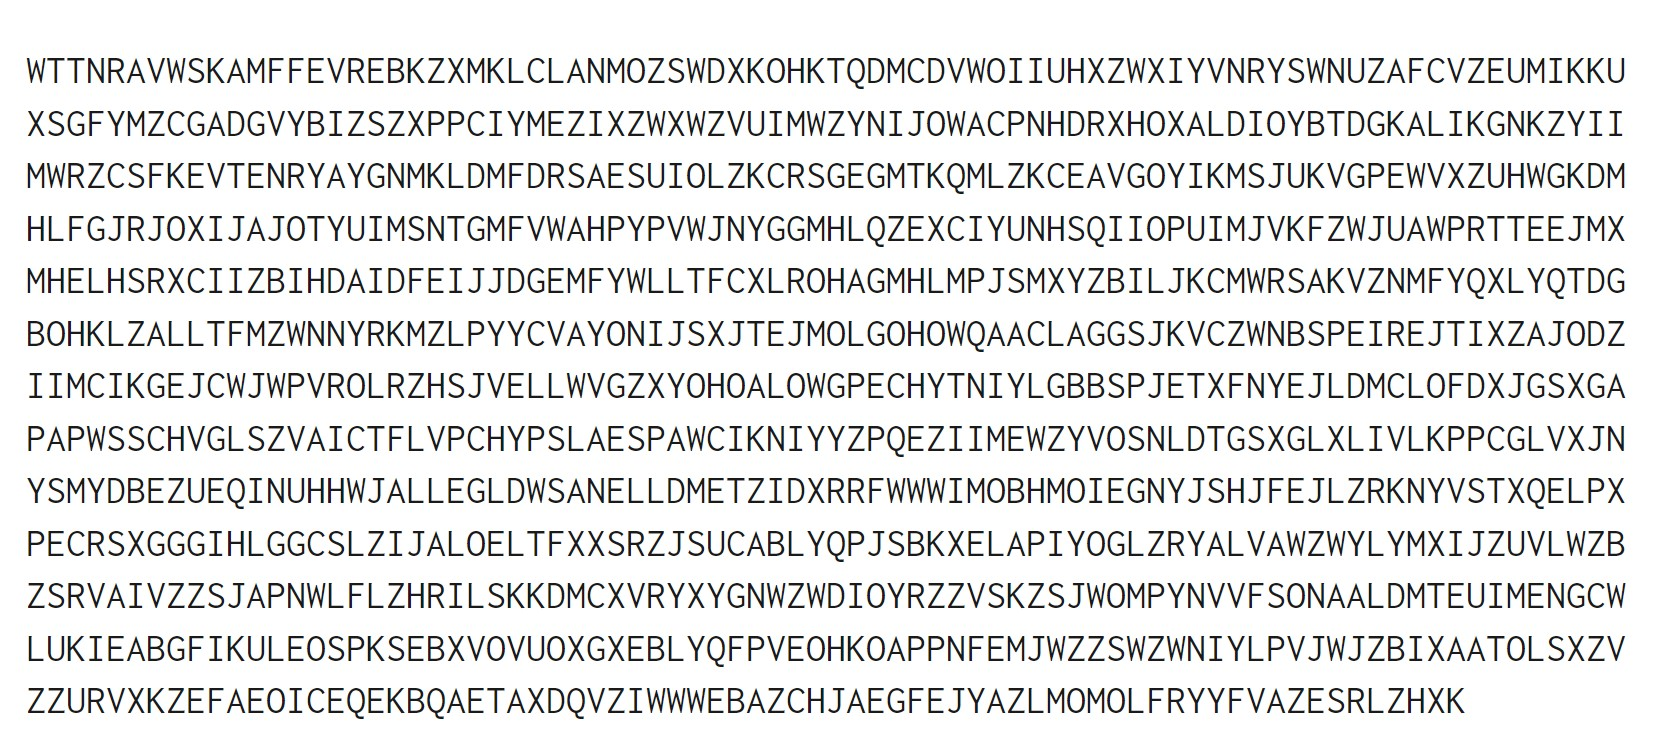
\includegraphics[scale = 0.7]{img/ex3.jpg}
        \label{ex3}
        % \caption{Friedman method: finding the key}
    \end{figure}
    
    \item Encrypt and decrypt message $(2,5)$ using the Hill cipher with $K =  \begin{bmatrix}
5 & 11 \\
8 & 3 
\end{bmatrix};$

    \item Encrypt and decrypt message $(1,3)$ using the Hill cipher with $K = \begin{bmatrix}
1 & 2 \\
4 & 3 
\end{bmatrix}$;

    \item Encrypt and decrypt message $(3,2)$ using the Hill cipher with $K = \begin{bmatrix}
3 & 1 \\
1 & 2 
\end{bmatrix}$

    Solution on slide 2 of L11;

    \item Suppose that we know that FRIDAY has been encrypted as PQCFKU using the Hill cipher, so we have (FRIDAY, PQCFKU). What is the key $K$? Assume $K$ is a 2x2 matrix. Solution on slide 29 of L5;

    \item Compute $\text{gcd}(17,2)$;

    \item Suppose $X = \begin{bmatrix}
5 & 17 \\
8 & 3 
\end{bmatrix}$ and $Y = \begin{bmatrix}
15 & 16 \\
2 & 5 
\end{bmatrix}$. We know that if $X^{-1}$ exists, then $K = X^{-1}Y \mod 26$. Compute $X^{-1}$ using the extended euclidean algorithm and retrieve $K$. Solution on slides 34-35-36 of L5;

    \item Compute $\text{EuclidExt}(14,17)$;

    \item Compute $\text{EuclidExt}(17,5)$. Solution on slide 38 of L5;

    \item Decrypt the following ciphertext, which was encrypted using a \textit{shift cipher}: BEEAKFYDJXUQYHYJIQRYHTYJIQFBQDUJIIKFUHCQD. Solution on slide 27 of L5;

    \item Try to break the following ciphertext encrypted with the autokey cipher: GUAAMLXOOVTMRVTKXOWSSDXNVJSTVTACALTNQFTPNIHUXRPWLV;

    \item Try to extract the plaintext from this word encoded using the autokey cipher. Notice that we do not know the key $k$: FTPNIH. Solution on slide 31-32 of L6;

    \item Prove that the cipher with the following encryption function $E_k(x_1, .., x_d) = (x_1 + k, .., x_d + k) \mod 26$ is not perfect. Use both the formal definition and the theorem 1 discussed in class. Solution on slide 3-4 of L7;

    \item Consider the following cipher with:

    \begin{itemize}
        \item $P = \{a,b\}$;
        \item $K = \{k_1, k_2, k_3\}$;
        \item $C = \{1,2,3,4\}$;
        \item $E_{k_1}(a) = 1$, $E_{k_2}(a) = 2$, $E_{k_3}(a) = 3$, $E_{k_1}(b) = 2$, $E_{k_2}(b) = 3$, $E_{k_3}(c) = 4$
    \end{itemize}

    We now let $p_p(a) = 1/4$, $p_p(b) = 3/4$, $p_{k}(k_1) = 1/2$, $p_{k}(k_2) = p_k(k_3) 1/4$. Compute $p_p(a|1)$, $p_p(a|2)$, $p_p(a|3)$, $p_p(a|4)$, $p_p(b|1)$, $p_p(b|2)$, $p_p(b|3)$, $p_p(b|4)$.
    
\end{enumerate}